

\section{Reset-VASS and state-resilience}\label{appendix}


% \section{Proof of Theorem~\ref{liveness reset}}\label{appendix}

% Recall Theorem~\ref{liveness reset}.


%\begin{proposition}\label{liveness reset}
% The  zero reachability problem can be reduced to the $t$-liveness problem in reset-VASS.
%\end{proposition}

Let us recall the {\em zero-reachability} problem in (reset-)VASS.

\noindent
input: a $d$-reset-VASS $V=(Q,T)$, and $p(\textbf{u}) \in Q \times \N^d$ \\
question:  $\exists q \in Q ~ p(\textbf{u}) \to^* q(\textbf{0})$ ?

The zero-reachability problem is decidable in VASS and it is undecidable in reset-VASS \cite{araki1976PN}.
%%%%%
\iffalse
%%%%
Let us recall the undecidable \cite{araki1976PN} decision problem of {\em zero-reachability} in reset-VASS, which consists in, given a
reset-VASS $V=(Q,T)$, and $p(\textbf{u}) \in Q \times \N^d$,
deciding whether $\exists q \in Q ~ p(\textbf{u}) \to^* q(\textbf{0})$.
%%
\fi
%%%%

For the sake of clarity \alain{bof, une autre raison?}, we will use reset Petri nets \cite{dufourd1998reset} rather than reset-VASS. 

A \emph{reset Petri net} $N = (\Pi, \Sigma, E, R, \mu)$ consists of a finite set of {\em places} $\Pi = \{r_1, r_2, ... r_{|\Pi|}\}$, a finite set of {\em transitions} $\Sigma = \{t_1, t_2, ..., t_{|\Sigma|} \}$, a finite set of {\em arcs} $E \subseteq \Pi \times \Sigma \cup \Sigma \times \Pi$, a finite set of
{\em reset-arcs} $R \subseteq \Sigma \times \Pi$, and an {\em initial marking} $\mu : \Pi \to \N$.
\alain{pourquoi ces notations étranges ? note N=(P,T,...) comme pour les Petri normaux et pas r les places, et pas sigma les transitions,...}
It is well-known that Petri nets and VASS are equivalents models with regards of the decidability of reachability problems: an $d$-VASS can be encoded into a Petri net with $d+2$ places and conversely, a Petri net with $p$ places can be encoded into a $p$-VASS~\cite{DBLP:journals/siglog/Schmitz16}. The same equivalence hold between reset-VASS and reset Petri nets.


We describe therein how to adjust Theorem~5.5 \alain{que dit le theorem 5.5 ?}\mathieu{reachability se réduit à liveness pour les Petri nets}from \cite{peterson1981petri} reducing the {\em zero-reachability} problem to {\sc $t$-liveness} in reset Petri nets. \\


\noindent
\textbf{Proposition~\ref{liveness reset}}
%\label{liveness reset}
{\em In reset Petri nets, the zero reachability problem can be reduced to {\sc $t$-liveness}.}



\begin{proof}


If we wish to determine if a marking in which every place is empty is reachable for a reset Petri net
 $N_1 = (\Pi_1, \Sigma_1, E_1, R_1, \mu_1)$ % with initial marking $\mu_1$, 
 we construct a reset Petri net
 $N_2 = (\Pi_2, \Sigma_2, E_2, R_2, \mu_2)$ % with initial marking $\mu_2$
  which is live if and only if the {\em zero marking}, which assigns $0$ to every place of $\Pi_1$, is not reachable from $\mu_1$ in $N_1$. \\

\begin{samepage}
{\bf Construction of $N_2$} \\
\indent
The reset Petri net $N_2$ is constructed from $N_1$ by the addition of two places $p_1$ and $p_2$ and $|\Pi_1| +2$ transitions $t_{p_1}$, $\{ t_p \mid p \in P_1 \}$ and $t_{p_2}$.
We first modify all transitions of $N_1$ to include $p_1$ as both an input and an output.
The initial marking $\mu_2$ will include a token in $p_1$ and no token in $p_2$. 
This new place $p_1$ serve to mark that the run is ongoing. As long as it contains a token, the adjusted transitions of $N_1$ are live and can be used normally. Thus any marking which is reachable in the places of $N_1$ is also reachable in the corresponding places of $N_2$.
We add an additional transition $t_{p_1}$ %\alain{s est d'habitude un état}
which has $p_1$ as an input and a null output.
This allows to disable the transitions of $N_1$ and to "freeze" the marking of the places of $\Pi_1$ in $N_2$.
 The place $p_1$ and transition $t_{p_1}$ allow the net $N_2$ to reach any reachable marking in $N_1$ and then for $t_{p_1}$ to fire and freeze the net at that marking.
We introduce a new place $p_2$ and new transitions $t_p$, for all $p \in \Pi_1$, which have $p$ as input and $p_2$ as output.
Lastly, we add a transition $t_{p_2}$ with $p_2$ as its output and every place of $\Pi_2$ as output, which ``floods'' the net with tokens, assuring that every transition is live if a token is ever
put in $p_2$.
\end{samepage}

 \begin{center}
	\begin{figure}
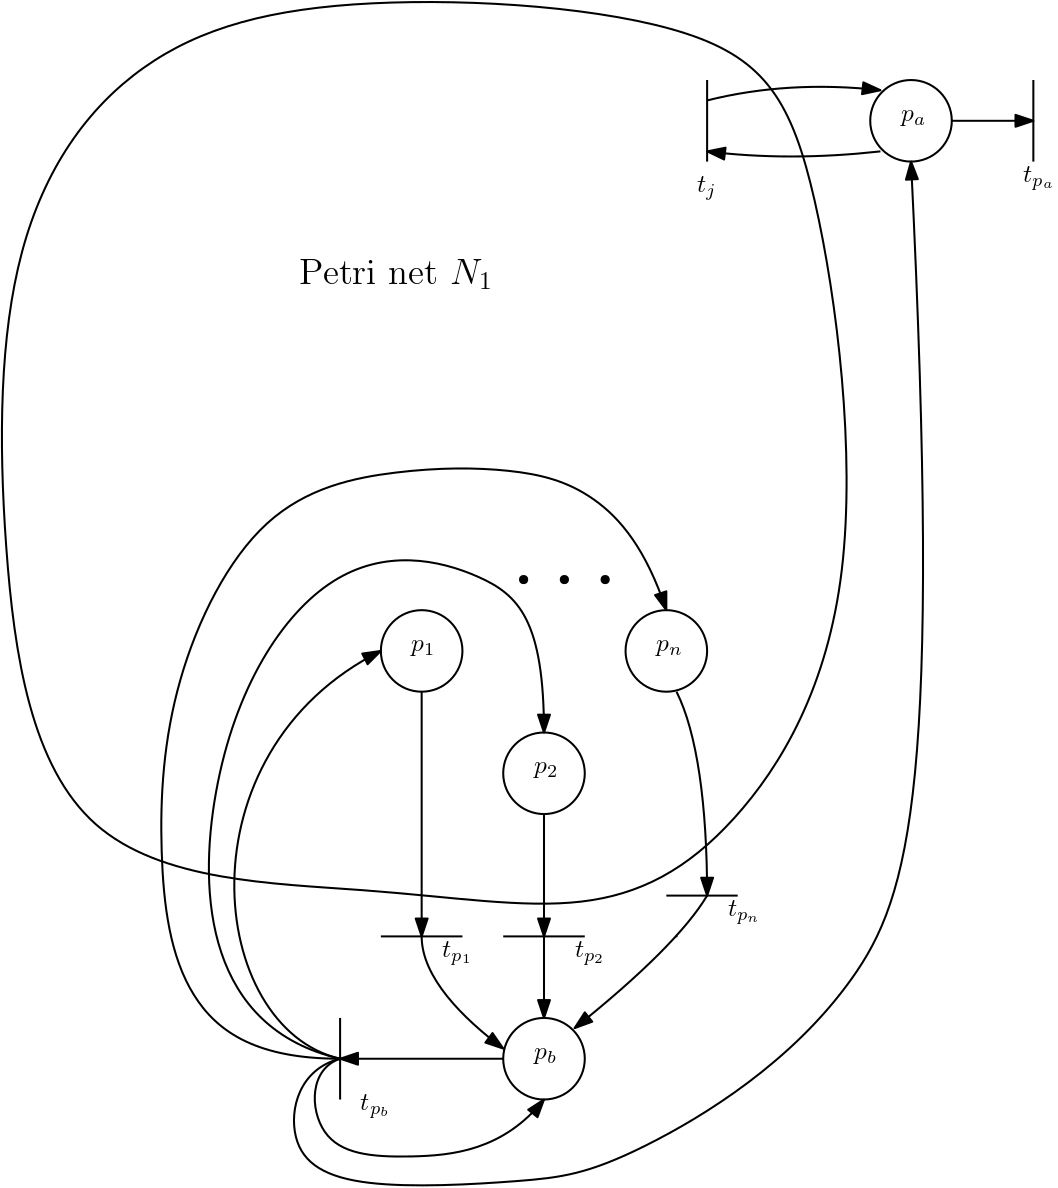
\includegraphics[width=0.75\textwidth]{FigurePN}
\caption{Construction of $N_2$ from $N_1$.}
	\end{figure}
\end{center}


Let us now prove that $t_2$ is live if and only if 
the zero marking
is not reachable from $\mu_1$ in $N_1$. \\


{\bf Suppose that the zero marking is reachable from $\mu_1$ in $N_1$, then $t_{p_2}$ is not live}

Indeed the marking with zero in every place of $\Pi_1$ and in $p_2$ is reachable in $N_2$, by executing the same sequence of transition firings. Then $t_{p_1}$ can fire, leading to the marking which assigns zero to every place of $\Pi_2$. From this marking the transitions $t_p$ are not live and neither are the transitions inherited from $N_1$ nor $t_{p_1}$, and, finally, nor is $t_{p_2}$. Thus $t_{p_2}$ is not live. \\


{\bf Suppose that $t_{p_2}$ is not live, then the zero marking is reachable from $\mu_1$ in $N_1$}

Indeed, if $t_{p_2}$ is not live, then a marking $\mu$ must be reachable in which $\mu(p_2) = 0$ and there is no reachable state in which $p_2$ has a token (in particular, since we do not allow token removal from $p_2$, the marking $\mu$ must be reached in a sequence of transitions that do not place any token in $p_2$).
This means that no transition $t_p$ is live in $\mu$ since any transition $t_p$ can place a token in $p_2$. 
Thus, every place of $\Pi_2$ inherited from $N_1$ must be devoid of token. Moreover, since the marking $\mu$ must be reached  in a sequence of transitions that do not place any token in $p_2$, 
it can be reached without using the transitions $t_p$ or $t_{p_2}$. Since $t_{p_1}$ do not modify the places inherited from $\Pi_1$ nor does it enable new transitions, the reachability of $\mu$ implies the reachability of a marking where every place of $\Pi_2$ inherited from $\Pi_1$ is devoid of token using only the transitions inherited from $N_1$. Thus the zero marking is reachable from $\mu_1$ in $N_1$.
\end{proof}

\alain{numérotation à faire}
\noindent
\textbf{Corollary~\ref{liveness reset VASS}}
%\label{liveness reset}
{\em In reset-VASS, the zero reachability problem can be reduced to {\sc $t$-liveness}.}







